\documentclass[conference]{IEEEtran} % or another class, depending on your target conference

% Packages
\usepackage{graphicx} % For including images
\usepackage{amsmath}  % For mathematical formulas
\usepackage{hyperref} % For hyperlinks
\usepackage{cite}     % For handling citations
\usepackage{caption}  % For customizing captions


% Title
\title{Multi-Step Object Re-Identification on Edge Devices: A Pipeline for Vehicle Re-Identification}

% Author(s)
\author{
	\IEEEauthorblockN{Tomass Zutis, Anzelika Bureka, Janis Judvaitis, Janis Arents, Modris Greitans, Peteris Racinskis}
	\IEEEauthorblockA{
		Institute of Electronics and Computer Science, Latvia\\
		janis.arents@edi.lv
	}
}

% Document
\begin{document}
	
	% Title page
	\maketitle
	
	% Abstract
	\begin{abstract}
A method that leverages a multi-step process focused on extracting and using object features for object re-identification is described. The proposed pipeline includes steps such as: detecting an object, converting its features into a vector embedding, storing this embedding in a vector database, and then querying the database to find the same or similar objects based on their feature embeddings. This approach allows for the identification of the same object across different images or cameras, even in varying locations, such as in Vehicle Re-Identification scenarios. For situations where re-identification needs to happen in outdoor environments or on-the-go, implementing this process on edge devices becomes crucial. Therefore, multiple ways to tailor the pipeline and its outputs for edge devices are outlined and investigated. The presentation provides a detailed explanation of the pipeline’s structure and how it functions on edge devices, along with the experimental setup demonstrating its application, particularly in vehicle re-identification.
	\end{abstract}
	
	% Keywords
	\begin{IEEEkeywords}
		Re-Identification, Feature extractions, Vector embeddings, Neural networks, Edge devices, Vector 
		databases
	\end{IEEEkeywords}
	
	% Sections
	\section{Introduction}
%	Introduce the problem of vehicle re-identification and the challenges of implementing this on edge devices. Discuss the significance of efficient computation in real-time applications.

Monitoring and recognizing objects in photos and videos has long been a field of interest for many. It has also become a well researched topic ever since computer vision has accelerated it's possibilities, in the last decade especially  \cite{prince2012computer}.
% vajag rakstu par computer vision potential un possibilities, lkm jau vecaaku
 With computer vision came image classification, which helped us classify images based on the object depicted. That gave us the answer to the question: "What is the object in the image?" \cite{lu2007survey}.
 % Te rakstu par object classification
  Later on came great progress in object detection. That could answer the questions of: "Where are the objects in the image?" and "What are the objects in the image". These were great leaps forward if the job was to pay attention to only objects of a specific class and there were multiple of them in a frame. This was first and foremost fostered by the advancement of the Convolutional Neural Network (CNN) and its variants. \cite{du2018understanding}.
  
% Te varetu ieklaut atsauci uz kadu pirmo sasniegumu objektu detektesanaa un pateikt ka vot vini domaja ka tas bija sasniegums
 In this article, however, the authors are looking for a solution that could see these objects of a single class and distinguish between them, using the specific features that exist only for a single individual in a class.
% Te laikam vajag ielikt definiciju no kaada raksta:
 This problem is called object Re-Identification - widely regarded as a sub-problem of image retrieval \cite{li2019object}.In imagery from at least two different cameras, object Re-identification aims to correctly label the same individual after imaging conditions (like scene, lighting conditions, object pose and others) have changed. In fact, this could be repeated for a specific class in any number of scenes, where there are usually more of these class objects visible. These could be images of vehicles, people or even animals or simple in-animate objects that have great intra-class variations.
 
 We are also in a unique position where there is still a lot of research to be done on re-identification itself, however, at the same time we are faced with the need to tailor these solutions for edge computing to preserve relevance in global technology and research trends. This is because some of the most common applications of re-identification are in traffic and security that use network cameras and cloud computing \cite{barthelemy2019edge} \cite{wang2024efficient}.
 Cities are looking for edge-computing devices using computer vision and deep neural networks to track real-time events in the public space. With the development of the Internet of Everything (IoE), the number of smart devices connected to the internet, the volume of available video footage, and the influx of sensory data have made the large-scale accumulation of big data inevitable \cite{cao2020overview}. This is why fully automated systems are needed to process data and re-identify patterns and objects in the smart cities environment, for no human or group of humans can be employed to process all this data manually and more crucially - in real time.
 
 \begin{figure}[b]
 	\centering
 	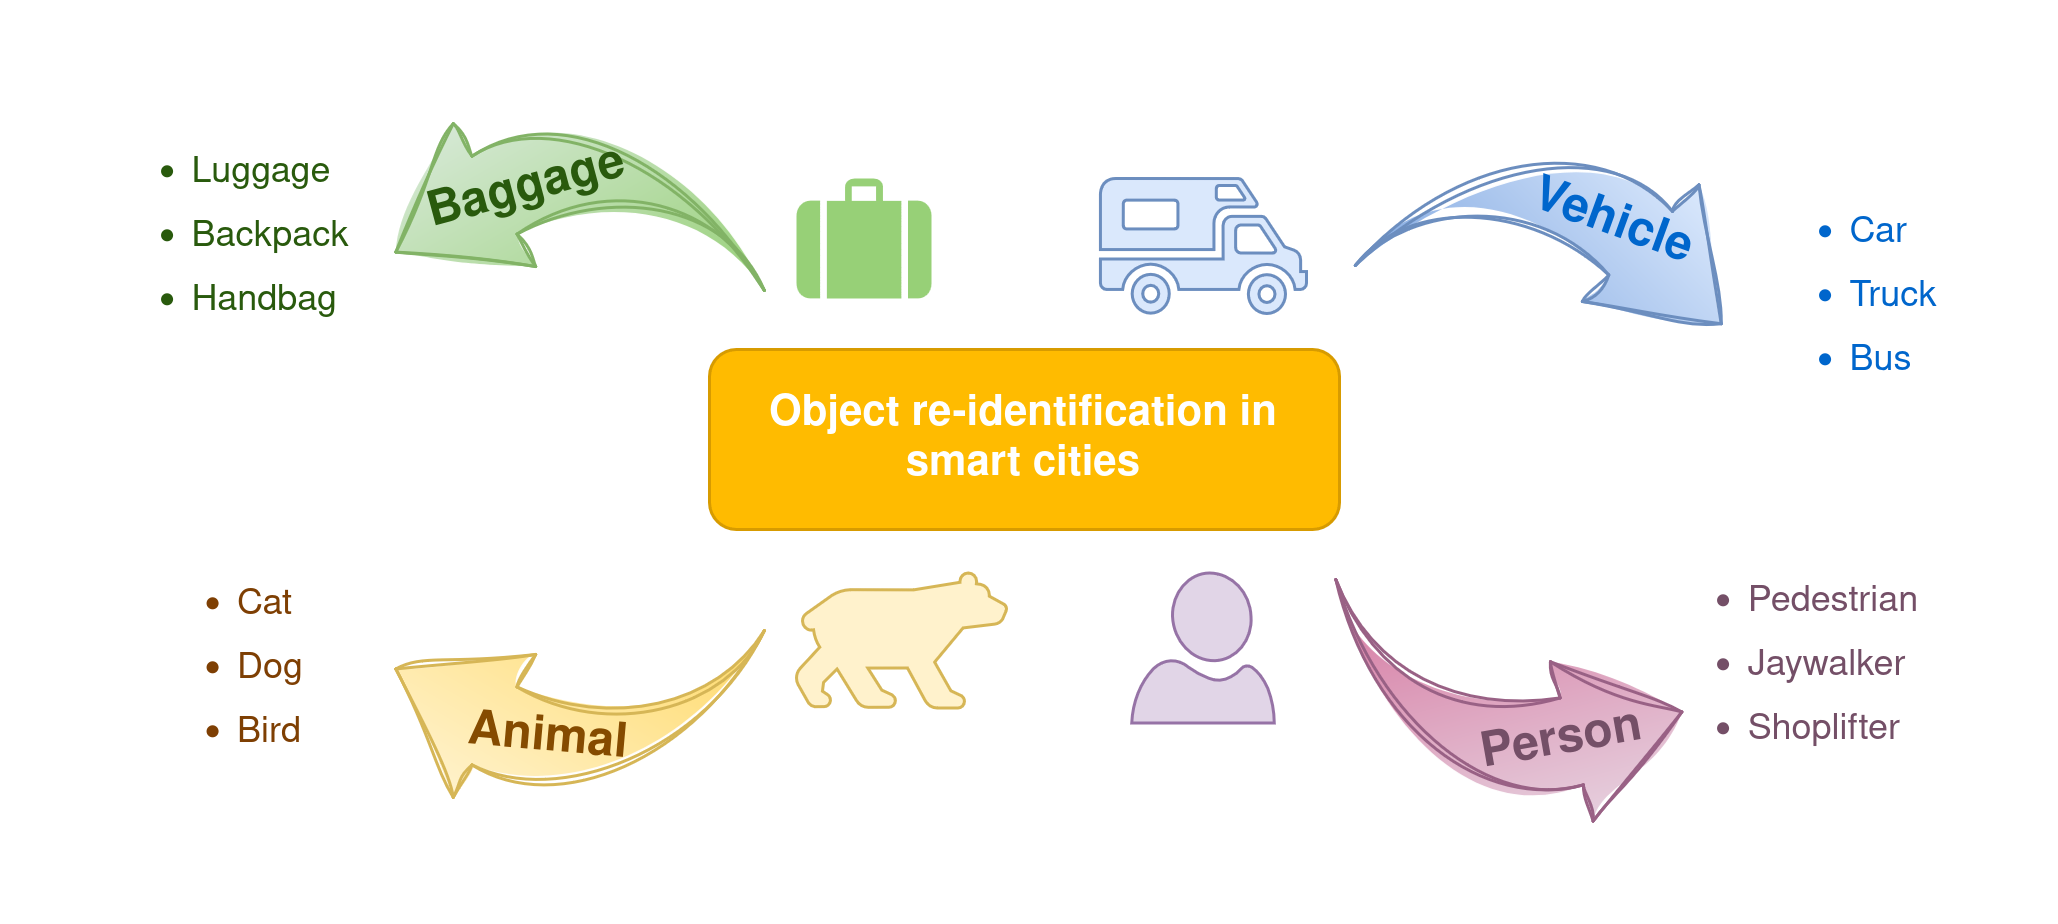
\includegraphics[width=0.5\textwidth]{re_id_diagramma_1.png} % Adjust width as needed
 	\caption{There are multiple uses for object re-identification in the smart cities context. Some of them are: people, vehicles, animals and even luggage in transit hubs.}
 	\label{fig:fig1} % Label for referencing the image
 \end{figure}
 
 In the scenario of traffic monitoring, there is the need to re-identify vehicles on the go to: first of all, be able to track them in a road network and, second, model future traffic based on the existing patterns \cite{barthelemy2019edge}. Edge computing proposes a hardware and software solution that would do this in real time - live video feed would be received from a network camera, that's deployed in the area of interest and the video analytics (i.e. detection and re-identification algorithms) are run directly on the edge device and only the results of the processing are transmitted.
 
 The natural solution to the object re-identification problem in these circumstances is a pipeline consisting of algorithms designed to cover all the necessary steps for re-identification to work. We argue that constructing a pipeline that receives live video feed, processes the frames to extract objects from each frame, saves these objects into memory and recognizes the same objects in a different scene's live video feed is possible and we aim to describe it in detail.
 
	
	\section{Related Work and State of the Art}
	
	Object re-identification to this day is heavily reliant on extracting robust feature representations for the objects we are trying to save. Differences in lighting, angle, occlusions, multiple models of the same object (vehicle) are an obstacle in getting reliable predictions \cite{kuma2019vehicle}. However, there is more to a working re-identification pipeline than just looking for the best way to produce vector embeddings. We have looked at the state of the art for multiple components of this problem, such ass: Object detection, Object re-identification and feature extractions, Person re-Identification, Vehicle re-identification, Available datasets, Synthetic datasets and Edge implementation.
	
	\subsection{Object detection}
	
	\section{Proposed Method}
%	Describe the steps of your multi-step pipeline for vehicle re-identification. Use equations and figures as needed.
%	\begin{itemize}
%		\item Object Detection
%		\item Feature Extraction
%		\item Vector Embedding with LanceDB
%	\end{itemize}
	
	\section{Experiments and Results}
%	Present the experiments, datasets, and evaluation metrics used to validate the method. Include tables, graphs, and illustrations.
	
	\section{Discussion}
%	Discuss the results and their implications. Highlight the future work on edge device implementation.
	
	\section{Conclusion}
%	Summarize the main findings of the paper and the significance of your work.
	
	% Bibliography
	\bibliographystyle{IEEEtran}
	\bibliography{references} % Make sure you have a .bib file with your references
	
\end{document}
